\documentclass[12pt]{article}
\usepackage[utf8]{inputenc}
\usepackage[T2A]{fontenc}
\usepackage[russian]{babel}
\usepackage{amsmath}
\usepackage{amssymb}
\usepackage{dsfont}
\usepackage[dvipsnames]{xcolor}
\usepackage{setspace}
\usepackage{multirow}
\usepackage[a4paper, outer=1.5cm, inner=1.5cm, top=1cm, bottom=1cm]{geometry}
\usepackage{graphicx}
\usepackage{skull}
\usepackage{wasysym}
\usepackage{float}
\graphicspath{{.images/}}
\usepackage{hyperref}
\hypersetup{colorlinks=true, linkcolor=blue, filecolor=magenta, urlcolor=cyan}
\usepackage[firstpage]{draftwatermark}
\SetWatermarkText{
    $\qquad\qquad\qquad\qquad\qquad$\parbox{7cm}{\begin{center}
    
\includegraphics[width = 0.08\textwidth]{lion-logo.png}\bigskip\\~\bigskip\\~\vspace{-24mm}\\~\end{center}}
}
\SetWatermarkAngle{0}
\SetWatermarkScale{1.5}
\usepackage{etoolbox}

\newtoggle{ifsolved}
\newtoggle{needhelp}
\newcounter{num}
\setcounter{num}{1}

\newcommand{\newnum}{\par\textbf{\textnumero\arabic{num}}\stepcounter{num}}
\newcommand{\sol}{\vspace{3mm}\par\textbf{Решение: }}
\newcommand{\ans}{\vspace{3mm}\par\textbf{Ответ: }}
\newcommand{\hint}{\vspace{3mm}\par\textbf{Подсказка: }}
\newcommand{\mode}[1]{
\ifstrequal{#1}{0}{\togglefalse{ifsolved}\togglefalse{needhelp}}{\ifstrequal{#1}{1}{\togglefalse{ifsolved}\toggletrue{needhelp}}{\ifstrequal{#1}{2}{\toggletrue{ifsolved}\togglefalse{needhelp}}{\toggletrue{ifsolved}\toggletrue{needhelp}}}}} %if 0 - if 1 - if 2 - else
%\newenvironment{problem}[8]{%#1, #2, #3
%\parbox{\linewidth}{\vspace{4mm}\ifstrequal{#4}{(лёгкая)}{\newnum\textbf{.}}{\newnum\textbf{*.} } \\ #5}
%\iftoggle{ifsolved}{\sol #6}{}
%\iftoggle{ifsolved}{\ans #7}{}
%\iftoggle{needhelp}{\hint #8}{}}

\newenvironment{problem}[8]{%#1, #2, #3
\parbox{\linewidth}{\vspace{5mm}\ifstrequal{#4}{(лёгкая)}{\newnum\textbf{.}}{\newnum\textbf{*.} } \\ #5}
\iftoggle{ifsolved}{\sol #6}{}

\iftoggle{ifsolved}{\parbox{\linewidth}{\ans #7}}{}
\iftoggle{needhelp}{\parbox{\linewidth}{\hint #8}}{}}

\newenvironment{mylist} %custom list
{ \begin{itemize}
    \setlength{\itemsep}{0pt}
    \setlength{\parskip}{0pt}
    \setlength{\parsep}{0pt}     }
{ \end{itemize}                  }

\newenvironment{homeass}[1]{\vspace*{-1.5cm}
\iftoggle{ifsolved}{
    \section*{\center{Решение домашнего задания к #1.}}
}{
    \section*{\center{\textcolor{Sepia}{Домашнее задание к #1}}}
} \vspace{7mm}\large}

\parindent=0pt
\pagestyle{empty}
%$\!$[\arabic{class}.\arabic{num}]
%\ifnumcomp{\value{counter}}{>}{1}{true}{false}
%\definecolor{Gray}{gray}{0.9}
%\definecolor{mypink}{RGB}{219, 48, 122}
%\newcolumntype{g}{>{\columncolor{Gray}}p{2.8cm}}

\begin{document}
\large
\mode{7}
%0 for problems without hints
%1 for problems + hints
%2 for problems + solutions + answers
%else: show all

{\centering\section*{СПИСОК ЗАДАЧ}}

{\centering\subsection*{\smallskip\\\textcolor{green}{\textbf{Полезные вещи, которые можно и нужно копипастить:}}}}

\subsection*{\textcolor{Emerald}{\textbf{Полезные шпаргалки по LaTeXу:}}}

\textbf{Пример вставки рисунка:}

\begin{minipage}{\linewidth}
    \begin{minipage}{0.54\linewidth}
    см. рисунок справа\\
    Текст к собственно пикче, примерно всегда это либо развёрнутое описание, либо большая часть решения задачи --- стремимся экономить пространство, если это можно сделать.
    \end{minipage}
    \hspace{0.05\linewidth}
    \begin{minipage}{0.4\linewidth}
    \begin{figure}[H] 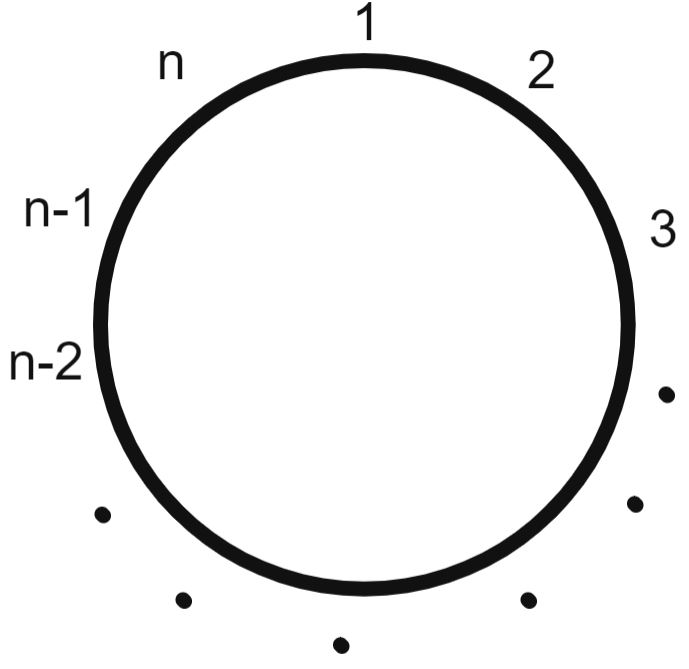
\includegraphics[width=\linewidth]{sol3} %тут поменять имя пикчи
    \end{figure}
    \end{minipage}
\end{minipage}

\textbf{Дефолтные математические знаки и символы:}\\
$\geqslant$,
$\leqslant$,
$a^{b}$,
$x_{i}$,
$\sqrt{a}$,
$\frac{a}{b}$,
$\displaystyle \frac{a}{b}$,
$\cdot$
$\;\Rightarrow\;$,
$\;\Leftrightarrow\;$,
$1{,}2$.
О промежутках:
$a\!b$,
$a\,b$,
$a\:b$,
$a\;b$,
$a\quad b$.

\textbf{Стандартные система и совокупность уравнений / неравенств:}\\
$\left\{
\begin{aligned}
f(x) &= 0 \\
g(x) &= 1
\end{aligned}\right.$

$\left[\begin{aligned}
&\left\{\begin{aligned}
f(x) &\geqslant a \\
g(x) &= b
\end{aligned}\right.\\
&\left\{\begin{aligned}
f(x) &< a \\
g(x) &= -b
\end{aligned}\right.
\end{aligned}\right.$

\subsection*{\textcolor{Emerald}{\textbf{Не математическое, но полезное:}}}
% комментарий в любом месте документа, который нигде не будет видно. Можно использовать для написания заметок-вопросов по задачам
\textbf{Пример таблицы:}

\begin{tabular}{|c|c|c|}
\hline
    $a$ & $b$ & текст
\\\hline
    $c$ & $d$ & мораль
\\\hline
\end{tabular}\\

\textbf{Отступы:} между\smallskip\\ строками\medskip\\ \textbf{Тире} --- это три дефиса.\\
\textbf{Списки:}
\begin{mylist}
\item [$\bullet$] это был пункт а
\item [2)] а это уже пункт номер 2 с изменённым заголовком
\end{mylist}

\subsection*{\textcolor{Emerald}{\textbf{Всё, неупомянутое выше (или если просто что-то не так):}}}
\begin{mylist}
\item [$\bullet$] Решение отдельных вопросов касательно ТеХа нужно искать в \href{https://www.mccme.ru/free-books/llang/newllang.pdf}{Львовском}.

\item [$\bullet$] Найти произвольный символ, который нужен, можно в \href{http://detexify.kirelabs.org/classify.html}{Detexify}.

\item [$\bullet$] Если возникли сомнения при решении, ответ практически ко всем задачам можно проверить с помощью \href{https://www.wolframalpha.com/}{WolframAlpha}.

\item [$\bullet$] Если в задаче нужно создать картинку, то лучше пока отложить эту задачу. Все графики планируется централизованно нарисовать (или перерисовать) в геогебре.

\item [\textcolor{brown}{\textbf{!!}}] Важно ставить \textcolor{red}{\textbf{$\spadesuit$}}
(или просто red) в тело задачи в случае серьёзных вопросов к решению и какой-то вопиющей лажи.

\item [\textcolor{brown}{\textbf{!!}}] Важно ставить \textcolor{olive}{\textbf{$\spadesuit$}}
(или просто olive) в тело задачи в случае не самого удачного текста и кривых отступов.
\end{mylist}

\subsection*{\textcolor{Violet}{\textbf{Комментарии:}}}% а также невидимые комментарии - так можно оставлять заметки-вопросы прямо в задаче, чтобы потом было понятно, в чём вопрос.
\begin{mylist}
\item [$\skull$] Переставлять задачи местами --- очень плохая идея.

\item [$\smiley$] При двойном клике по тексту pdf справа происходит автоматический переход к этому месту в латех-коде, а для обратного перехода можно нажать стрелку вправо (висит сверху между pdf и латех-кодом).

\item [$\smiley$] Если есть размышления, дописывать red/olive к задаче или не дописывать, то лучше всё-таки дописать.

\item [$\skull$] Самое плохое, что можно сделать --- написать в любое поле из трёх (НаписанноеРешение/ВерныйОтвет/Подсказка) только половину того, что надо, никак это не отметить, и потом пойти дальше.\\ Нужно в этот момент писать red/olive в случайном месте задачи, чтобы потом вычислить это с помощью Ctrl+F по всему документу (и это то, что потом будет делаться долго и тщательно)
\end{mylist}

\newpage
\setcounter{num}{731}

\hypertarget{7.8}{{\centering\section*{\bigskip\\\textcolor{Blue}{\hyperlink{start2}{\textcolor{Blue}{7.8}} Алгебраические дроби.}\vspace{-5mm}}}}

\begin{problem}{Основные понятия.}{7.8.1}{6K}{(лёгкая)}
{Правда ли, что $\displaystyle\frac{2p + 2}{p + 1}$ = 2?}
{НаписанноеРешение}
{ВерныйОтвет}{Подсказка}
\end{problem}

\begin{problem}{Сложение и вычитание алгебраических дробей.}{7.8.2}{79I}{(лёгкая)}
{Известно, что $\displaystyle\frac{a}{b} = 3$. Найти значение выражения $\displaystyle\frac{2a - 3b}{a}$.}
{НаписанноеРешение}
{ВерныйОтвет}{Подсказка}
\end{problem}

\begin{problem}{Сложение и вычитание алгебраических дробей.}{7.8.2}{79I}{(лёгкая)}
{Сумма чисел $a$ и $b$, не равных нулю, равна их произведению.\\ Чему равно значение выражения $\;\frac{1}{2a} + \frac{1}{2b}$?}
{Чтобы сложить дроби, нужно их привести к общему знаменателю. Значит, $\frac{1}{2a} + \frac{1}{2b} = \frac{b}{2ab} + \frac{a}{2ab} = \frac{a + b}{2ab}$. Тут как раз в числителе --- сумма чисел $a$ и $b$, а в знаменателе --- их произведение. Если они равны, то это одно и то же число (и по условию это не ноль). Значит, на это число дробь можно сократить: $\;\frac{a + b}{2ab} = \frac{1}{2}$.}
{При таких условиях $\frac{1}{2a} + \frac{1}{2b} = \frac{1}{2}$.}{Приведи дроби к общему знаменателю. Что оказалось в числителе?}
\end{problem}

\begin{problem}{Умножение и деление алгебраических дробей.}{7.8.3}{7A}{(лёгкая)}
{Вычислить значение выражения $\;\displaystyle (a^{3} - 16a) \cdot \left(\frac{1}{a + 4} - \frac{1}{a - 4}\right)$ при $a = -15$.}
{Прежде чем вычислять значение выражения, упростим его.\\ Для начала найдём разность двух алгебраических дробей в скобках: для этого нужно привести их к общему множителю, а значит, домножить первую дробь на $a - 4$, а вторую --- на $a + 4$. Получаем: $\displaystyle (a^{3} - 16a) \cdot \left(\frac{a - 4}{(a + 4)(a - 4)} - \frac{a + 4}{(a - 4)(a + 4)}\right) =$
$\displaystyle (a^{3} - 16a) \cdot \left(\frac{a - 4 - (a + 4)}{(a + 4)(a - 4)}\right) = \displaystyle (a^{3} - 16a) \cdot \left(\frac{-8}{a^2 - 16}\right)$. Таким образом, выражение в скобках найдено и ясно, что полученный результат можно сократить ещё: $$(a^{3} - 16a) \cdot \left(\frac{-8}{a^2 - 16}\right) = a\cdot(a^2 - 16) \cdot \frac{-8}{a^2 - 16} = \frac{-8a \cdot \textcolor{violet}{(a^2 - 16)}}{\textcolor{violet}{(a^2 - 16)}} = -8a.$$
Это упрощать уже некуда, но ведь $a = -15$, а значит $-8a = (-8)(-15) = 120$.}
{$\displaystyle (a^{3} - 16a) \cdot \left(\frac{1}{a + 4} - \frac{1}{a - 4}\right) = -8a = 120$ (при $a = -15$).}{Найди разность дробей и сократи получившуюся дробь.}
\end{problem}

\begin{problem}{Степень с произвольным целым показателем.}{7.8.4}{7A}{(лёгкая)}
{Вычислить значение выражения $\,\displaystyle a^{-3}$ при $a = \frac{1}{2}$.}
{НаписанноеРешение}
{ВерныйОтвет}{Подсказка}
\end{problem}

\begin{problem}{Степень с произвольным целым показателем.}{7.8.4}{7A}{(лёгкая)}
{Вычислить значение выражения $\,\displaystyle c^{-3} : c^{-4}$ при $c = 7$.}
{НаписанноеРешение}
{ВерныйОтвет}{Подсказка}
\end{problem}

\begin{problem}{Тождественные преобразования-1.}{7.8.5}{79I}{(лёгкая)}
{Упростить и вычислить: $\:\displaystyle \frac{3\cdot 116 - 5\cdot58}{29\cdot8}$.}
{НаписанноеРешение}
{ВерныйОтвет}{Подсказка}
\end{problem}

\begin{problem}{Тождественные преобразования-1.}{7.8.5}{79I}{(лёгкая)}
{Упростить и вычислить: $\:\displaystyle \frac{2\cdot 91 - 26}{6\cdot5 - 12\cdot3 + 18\cdot1}$.}
{НаписанноеРешение}
{ВерныйОтвет}{Подсказка}
\end{problem}

\begin{problem}{Тождественные преобразования-1.}{7.8.5}{79I}{(лёгкая)}
{Выразить $w$ через $a, b, c, d, e$, если $\;\displaystyle\frac{a + b}{w - c + d} - \frac{a + b}{w + c - d} = e$.}
{НаписанноеРешение}
{ВерныйОтвет}{Подсказка}
\end{problem}

\begin{problem}{Тождественные преобразования-1.}{7.8.5}{79I}{(лёгкая)}
{Упростить выражение $\displaystyle\left(\frac{x + 2b}{x - 2b} + \frac{x + 2a}{x - 2a}\right) : \frac{x}{2}$, если $\displaystyle x = \frac{4ab}{a + b}$.}
{НаписанноеРешение}
{ВерныйОтвет}{Подсказка}
\end{problem}

\begin{problem}{Тождественные преобразования-1.}{7.8.5}{6K}{(лёгкая)}
{Найти значение выражения $\displaystyle\frac{p(a)}{p\left(\frac{1}{a}\right)}$ если $\displaystyle p(t) = \left(t + \frac{6}{t}\right) \cdot \left(6t + \frac{1}{t}\right)$\smallskip\\
Например, $p(1) = (1 + 6)(6 + 1) = 49$. Можно посчитать для какого-нибудь примера, например, $3$ и $1/3$. А потом думать...}
{НаписанноеРешение}
{ВерныйОтвет}{Подсказка}
\end{problem}

\begin{problem}{Тождественные преобразования-1.}{7.8.5}{79I}{(лёгкая)}
{Упростить выражение $\:\displaystyle \frac{3x^2 - 48}{x + 4}$.}
{НаписанноеРешение}
{ВерныйОтвет}{Подсказка}
\end{problem}

\begin{problem}{Тождественные преобразования-1.}{7.8.5}{79I}{(лёгкая)}
{Сократить дробь $\:\displaystyle \frac{2s - 2t}{s^2 - t^2}\:$ и найти условие, при котором дробь нельзя сократить.}
{Для того чтобы сократить дробь, разложим на множители и числитель, и знаменатель: $\frac{2s - 2t}{s^2 - t^2} = \frac{2(s - t)}{(s - t)(s + t)}$. Числитель и знаменатель дроби можно одновременно домножить или разделить на одно и то же число, если это число --- не ноль. Значит, если $s - t \neq 0$ ($s \neq t$), получаем, что наша дробь равна $\frac{2}{s + t}$.}
{$\displaystyle \frac{2s - 2t}{s^2 - t^2} = \frac{2}{s + t}$. $\;$ Дробь нельзя сокращать, если $s$ и $t$ равны.}{Разложи на множители и числитель, и знаменатель. Существует ли множитель, на который дробь сокращать нельзя?}
\end{problem}

\begin{problem}{Тождественные преобразования-1.}{7.8.5}{79I}{(лёгкая)}
{Упростить выражение $\:\displaystyle \frac{11}{7a - 14} + \frac{3}{4 - a^2}$.}
{НаписанноеРешение}
{ВерныйОтвет}{Подсказка}
\end{problem}

\begin{problem}{Тождественные преобразования-1.}{7.8.5}{79I}{(лёгкая)}
{Упростить выражение $\:\displaystyle \frac{2y^2 + 10y + 8}{y^2 + 3y + 2}$.}
{Чтобы упростить выражение, разложим и числитель, и знаменатель на множители. Для этого используем теорему Виета: для числителя сумма корней равна $-5$, произведение корней равно 4. Поэтому корни --- $-4$ и $-1$. Для знаменателя сумма корней равна $-3$, произведение корней равно 2. Корнями будут $-2$ и $-1$. Используем разложение $ax^2 + bx + c = a(x - x_1)(x - x_2)$ и получаем, что $$\frac{2y^2 + 10y + 8}{y^2 + 3y + 2} = \frac{2(y + 1)(y + 4)}{(y + 1)(y + 2)} = \frac{2y + 8}{y + 2}.$$}
{$\displaystyle \;\frac{2y^2 + 10y + 8}{y^2 + 3y + 2} = \frac{2y + 8}{y + 2}$.}{Разложи числитель и знаменатель на множители.\\ Можно использовать теорему Виета, метод группировки, или дискриминант.}
\end{problem}

\begin{problem}{Тождественные преобразования-1.}{7.8.5}{79I}{(лёгкая)}
{Упростить выражение $\:\displaystyle \frac{b^2 - 7b - 16}{b^2 + 4b + 3} + \frac{5}{b + 1} - \frac{b - 4}{b + 3}$.}
{Так как нам надо сложить дроби, выясним, что в знаменателе: по теореме Виета $\,b^2 + 4b + 3 = (b + 1)(b + 3)$. Таким образом получаем, что
$$\frac{b^2 - 7b - 16}{b^2 + 4b + 3} + \frac{5}{b + 1} - \frac{b - 4}{b + 3} = \frac{b^2 - 7b - 16}{b^2 + 4b + 3} + \frac{5(b + 3)}{b^2 + 4b + 3} - \frac{(b - 4)(b + 1)}{b^2 + 4b + 3} =$$
$$= \frac{b^2 - 7b - 16 + 5b + 15 -(b^2 - 3b - 4)}{(b + 1)(b + 3)} = \frac{b + 3}{(b + 1)(b + 3)} = \frac{1}{b + 1}.$$}
{$\:\displaystyle \frac{b^2 - 7b - 16}{b^2 + 4b + 3} + \frac{5}{b + 1} - \frac{b - 4}{b + 3} = \frac{1}{b + 1}$.}{Приведи дроби к общему знаменателю и сократи дробь.}
\end{problem}

\begin{problem}{Тождественные преобразования-1.}{7.8.5}{79I}{(лёгкая)}
{Упростить выражение $\displaystyle \frac{a^{3} + b^{3}}{a + b} : (a^{2} - b^{2}) + \frac{2b}{a + b} - \frac{ab}{a^{2} - b^{2}}$ и найти его значение при $a = \sqrt{33} + 2$, $b = \sqrt{55} - 4$.}
{Для упрощения выражения приведём дроби к общему знаменателю:
$$\frac{a^{3} + b^{3}}{a + b} : (a^{2} - b^{2}) + \frac{2b}{a + b} - \frac{ab}{a^{2} - b^{2}} = \frac{\textcolor{Emerald}{(a + b)}(a^2 - ab + b^2)}{\textcolor{Emerald}{(a + b)}(a^{2} - b^{2})} + \frac{2b}{a + b} - \frac{ab}{a^{2} - b^{2}} =$$
$$=\frac{a^2 - ab + b^2}{a^{2} - b^{2}} + \frac{2b(a - b)}{(a + b)(a - b)} - \frac{ab}{a^{2} - b^{2}} = \frac{a^2 - ab + b^2 + 2b(a - b) - ab}{a^2 - b^2} =$$
$$=\frac{a^2 - b^2}{a^2 - b^2} = 1.\quad \text{Таким образом, от $a$ и $b$ выражение не зависит} \to \text{ответ --- 1.}$$}
{$\displaystyle \frac{a^{3} + b^{3}}{a + b} : (a^{2} - b^{2}) + \frac{2b}{a + b} - \frac{ab}{a^{2} - b^{2}} = \frac{a^2 - b^2}{a^2 - b^2} = 1$.}{Приведи все дроби к общему знаменателю.}
\end{problem}

\begin{problem}{Тождественные преобразования-1.}{7.8.5}{79I}{(лёгкая)}
{Упростить выражение $\displaystyle \frac{a^{3} + a^{2} - a - 1}{a^{2} + 2a + 1}$ и найти его значение при $a = 11$.}
{Для того, чтобы упростить дробь --- а данное выражение представляет собой дробь, у которой и в числителе, и в знаменателе многочлены, надо её сократить. Для этого заметим в знаменателе квадрат суммы: $\frac{a^{3} + a^{2} - a - 1}{a^{2} + 2a + 1} = \frac{a^{3} + a^{2} - a - 1}{(a + 1)^2}$.\\
Воспользуемся методом группировки: $a^{3} + a^{2} - a - 1 = a^2(a + 1) - (a + 1) = (a + 1)(a^2 - 1)$. Теперь используем формулу разности квадратов: $(a + 1)(a^2 - 1) = (a + 1)\cdot(a - 1)(a + 1) = (a - 1)(a + 1)^2$. Итого, $\frac{a^{3} + a^{2} - a - 1}{(a + 1)^2} = \frac{(a - 1)(a + 1)^2}{(a + 1)^2} = a - 1$.\\
При $a = 11$ это равно 10.}
{$\;\displaystyle \frac{a^{3} + a^{2} - a - 1}{a^{2} + 2a + 1} = \frac{(a - 1)(a + 1)^2}{(a + 1)^2} = a - 1 = 11 - 1 = 10$.}{Для сокращения данной дроби разложи числитель и знаменатель на множители. Используй метод группировки.}
\end{problem}

\begin{problem}{Тождественные преобразования-1.}{7.8.5}{79I}{(лёгкая)}
{Упростить выражение $\displaystyle\left(\left(\frac{1}{a} + \frac{1}{b + c}\right):\left(\frac{1}{a} - \frac{1}{b + c}\right)\right) : \left(1 + \frac{b^{2} + c^{2} - a^{2}}{2bc}\right) $ и найти его значение при $a = 1\frac{33}{40}$, $b = 0{,}625$, $c = 3{,}2$.}
{НаписанноеРешение}
{ВерныйОтвет}{Подсказка}
\end{problem}

\begin{problem}{Тождественные преобразования-1.}{7.8.5}{79I}{(лёгкая)}
{Упростить выражение $\displaystyle\left(x^{2} + 2x - \frac{11x - 2}{3x + 1}\right) : \left(x + 1 - \frac{2x^{2} + x + 2}{3x + 1}\right)$ и найти его значение при $x = 7{,}(3)$.}
{НаписанноеРешение}
{ВерныйОтвет}{Подсказка}
\end{problem}

\begin{problem}{Тождественные преобразования-1.}{7.8.5}{79I}{(лёгкая)}
{Упростить выражение $\displaystyle\left(\cfrac{2 - b}{b - 1} + 2 \cdot \cfrac{a - 1}{a - 2}\right) : \left(b \cdot \cfrac{a - 1}{b - 1} + a \cdot \cfrac{2 - b}{a - 2}\right)$ и найти его значение при $a = \sqrt{2} + 0{,}8$, $b = \sqrt{2} - 0{,}2$.}
{НаписанноеРешение}
{ВерныйОтвет}{Подсказка}
\end{problem}

\begin{problem}{Тождественные преобразования-1.}{7.8.5}{79I}{(лёгкая)}
{Упростить выражение $\displaystyle \left(\frac{a}{b} + \left(\frac{a}{b}\right)^{-1} - 2\right) : \frac{-1 + (a + 1)(b + 1) - ab}{(a + b)^{2} - (a - b)^{2}}$ и найти его значение при $a = 56 + 78\sqrt{90}$, $b = 65 + 78\sqrt{90}$.}
{НаписанноеРешение}
{ВерныйОтвет}{Подсказка}
\end{problem}

\begin{problem}{Тождественные преобразования-1.}{7.8.5}{X}{(лёгкая)}
{Упростить выражение $\displaystyle \frac{4x + 4y}{x^{2} - y^{2}}$ и найти его значение при $x = 1{,}(23456789)$, \\$y = 11{,}(23456789)$.}
{Разложим на множители числитель и знаменатель: $4x + 4y = 4(x + y)$, $x^2 - y^2 = (x - y)(x + y)$ (разность квадратов). Таким образом, $\frac{4x + 4y}{x^{2} - y^{2}} = \frac{4(x + y)}{(x - y)(x + y)}$. Теперь дробь можно сократить на $(x + y)$, получаем $\frac{4}{x - y} = \frac{4}{1{,}(23456789) - 11{,}(23456789)} =$ $= \frac{4}{1 - 11} = \frac{4}{-10} = -0{,}4$.}
{$\;\displaystyle \frac{4x + 4y}{x^{2} - y^{2}} = \frac{4}{x - y} = -0{,}4$.}{Для сокращения данной дроби разложи числитель и знаменатель на множители.}
\end{problem}

\begin{problem}{Тождественные преобразования-1.}{7.8.5}{79I}{(лёгкая)}
{Найти значение выражения $\displaystyle \frac{(z - 1)(z + 2)(z - 3)(z + 4)}{23}$, если $\displaystyle z = \frac{\sqrt{3} - 1}{2}$.}
{НаписанноеРешение}
{ВерныйОтвет}{Подсказка}
\end{problem}

\begin{problem}{Тождественные преобразования-1.}{7.8.5}{79I}{(лёгкая)}
{Упростить выражение: $\;\displaystyle \left(m + n - \frac{4mn}{m + n}\right) : \left(\frac{m}{m + n} - \frac{n}{n - m} - \frac{2mn}{m^{2} - n^{2}}\right).$}
{Приведём каждое из выражений в скобках к общим знаменателям:
$$m + n - \frac{4mn}{m + n} = \frac{(m + n)^2}{m + n} - \frac{4mn}{m + n} = \frac{m^2 + 2mn + n^2 - 4mn}{m + n} = \frac{(m - n)^2}{m + n}.$$
$$\frac{m}{m + n} - \frac{n}{n - m} - \frac{2mn}{m^{2} - n^{2}} = \frac{m(m - n)}{m^2 - n^2} - \frac{n(n + m)}{n^2 - m^2} - \frac{2mn}{m^2 - n^2} = \frac{m(m - n)}{m^2 - n^2} + $$ $$\frac{n(n + m)}{m^2 - n^2} - \frac{2mn}{m^2 - n^2} = \frac{m^2 - mn + n^2 + nm - 2mn}{m^2 - n^2} = \frac{(m - n)^2}{m^2 - n^2} = \frac{m - n}{m + n}.$$
Таким образом, получаем $\displaystyle\;\frac{(m - n)^2}{m + n} : \frac{m - n}{m + n} = \frac{(m - n)^2}{m + n} \cdot \frac{m + n}{m - n} = m - n$.}
{$\displaystyle \left(m + n - \frac{4mn}{m + n}\right) : \left(\frac{m}{m + n} - \frac{n}{n - m} - \frac{2mn}{m^{2} - n^{2}}\right) = m - n$.}{Приведи и выражение в первых скобках, и выражение во вторых скобках к общим знаменателям. Сократи множители.}
\end{problem}

\begin{problem}{Тождественные преобразования-1.}{7.8.5}{79I}{(лёгкая)}
{Упростить выражение $\;\displaystyle\frac{ab - 2b - 6 + 3a}{a^{2} - 4}$.}
{НаписанноеРешение}
{ВерныйОтвет}{Подсказка}
\end{problem}

\begin{problem}{Тождественные преобразования-1.}{7.8.5}{79I}{(лёгкая)}
{Упростить выражение $\;\displaystyle\frac{6}{a - 1} - \frac{10}{(a - 1)^{2}} : \frac{10}{a^{2} - 1} - \frac{2a + 2}{a - 1}$.}
{Будем постепенно упрощать это выражение:
$$\frac{6}{a - 1} - \frac{10}{(a - 1)^{2}} : \frac{10}{a^{2} - 1} - \frac{2a + 2}{a - 1} = \frac{6}{a - 1} - \frac{10}{(a - 1)^{2}} \cdot \frac{a^{2} - 1}{10} - \frac{2a + 2}{a - 1} =$$
$$\frac{6}{a - 1} - \frac{a^{2} - 1}{(a - 1)^{2}} - \frac{2a + 2}{a - 1} = \frac{6}{a - 1} - \frac{(a + 1)(a - 1)}{(a - 1)^{2}} - \frac{2a + 2}{a - 1} = $$
$$ \frac{6}{a - 1} - \frac{a + 1}{a - 1} - \frac{2a + 2}{a - 1} = \frac{6 - (a + 1) - (2a + 2)}{a - 1} = \frac{3 - 3a}{a - 1} = \frac{-3(a - 1)}{a - 1} = -3.$$}
{Данное выражение равно $-3$ (и от значения $a$ совсем не зависит).}{Подели одну дробь на другую, сократи числитель и знаменатель, получи одну дробь с общим знаменателем.}
\end{problem}

\begin{problem}{Тождественные преобразования-1.}{7.8.5}{79I}{(не лёгкая)}
{Упростить выражение $\;\displaystyle\left(\left(\frac{x^{2}}{y^{3}} + \frac{1}{x}\right) : \left(\frac{x}{y^{2}} - \frac{1}{y} + \frac{1}{x}\right)\right):\frac{(x - y)^{2} 
+ 4xy}{1 + \frac{y}{x}}$.}
{$\displaystyle\left(\left(\frac{x^{2}}{y^{3}} + \frac{1}{x}\right) : \left(\frac{x}{y^{2}} - \frac{1}{y} + \frac{1}{x}\right)\right):\frac{(x - y)^{2} 
+ 4xy}{1 + \frac{y}{x}} =$
$$=\left(\left(\frac{x^{3}}{xy^{3}} + \frac{y^3}{xy^3}\right) : \left(\frac{x^2}{xy^{2}} - \frac{xy}{xy^2} + \frac{y^2}{xy^2}\right)\right):\frac{x^2 + 2xy + y^2}{1 + \frac{y}{x}} = $$
$$=\left(\frac{x^{3} + y^3}{xy^3} : \frac{x^2 - xy + y^2}{xy^2}\right):\frac{x\cdot(x^2 + 2xy + y^2)}{x\cdot(1 + \frac{y}{x})} =$$ $\displaystyle\left(\frac{(x + y)(x^2 - xy + y^2)}{xy^3} \cdot \frac{xy^2}{x^2 - xy + y^2}\right) : \frac{x\cdot(x + y)^2}{x + y} = \frac{x + y}{y} \cdot \frac{1}{x\cdot(x+y)} = \frac{1}{xy}$.}
{$\displaystyle\left(\left(\frac{x^{2}}{y^{3}} + \frac{1}{x}\right) : \left(\frac{x}{y^{2}} - \frac{1}{y} + \frac{1}{x}\right)\right):\frac{(x - y)^{2} 
+ 4xy}{1 + \frac{y}{x}} = \frac{1}{xy}$.}{Приведи суммы и разности дробей к общим знаменателям.\\ Практически всё сократится.}
\end{problem}

\begin{problem}{Тождественные преобразования-1.}{7.8.5}{79I}{(лёгкая)}
{Упростить выражение $\;\displaystyle \frac{(a - b)^{2} + ab}{(a + b)^{2} - ab} : \frac{a^{5} + b^{5} + a^{2}b^{3} + a^{3}b^{2}}{(a^{3} + b^{3} +a^{2}b + ab^{2})(a^{3} - b^{3})}$.}
{НаписанноеРешение}
{ВерныйОтвет}{Подсказка}
\end{problem}

\begin{problem}{Тождественные преобразования-1.}{7.8.5}{79I}{(лёгкая)}
{Упростить выражение $\;\displaystyle\left(2 - x + 4x^{2} + \cfrac{5x^{2} - 6x + 3}{x - 1}\right) : \left(2x + 1 + \cfrac{2x}{x - 1}\right)$.}
{НаписанноеРешение}
{ВерныйОтвет}{Подсказка}
\end{problem}

\begin{problem}{Тождественные преобразования-1.}{7.8.5}{79I}{(лёгкая)}
{Упростить выражение $\;\displaystyle \left(\frac{2x - 1}{x^{2} + 2x + 4} + \frac{1}{x - 2} + \frac{9x + 6}{x^{3} - 8}\right) \cdot \frac{x^{2} - 4}{9}$.}
{Чтобы сложить дроби (а это надо сделать до умножения), нужно привести их к общему знаменателю. При разложении на множители для третьей дроби используем формулу разности кубов: $x^3 - 8 = (x - 2)(x^2 + 2x + 4)$. Становится понятно, что это и есть общий знаменатель этих трёх дробей. Таким образом,
$\displaystyle \frac{2x - 1}{x^{2} + 2x + 4} + \frac{1}{x - 2} + \frac{9x + 6}{x^{3} - 8} = \frac{(2x - 1)(x - 2)}{x^{3} - 8} + \frac{x^2 + 2x + 4}{x^{3} - 8} + \frac{9x + 6}{x^{3} - 8} = $\\
$\displaystyle = \frac{2x^2 - 5x + 2 + x^2 + 2x + 4 + 9x + 6}{x^{3} - 8} = \frac{3x^2 + 6x + 12}{x^{3} - 8} = \frac{3(x^2 + 2x + 4)}{x^{3} - 8} = \frac{3}{x - 2}$\smallskip\\
Итого, осталось перемножить две дроби: $\displaystyle \frac{3}{x - 2} \cdot \frac{x^2 - 4}{9} = \frac{x + 2}{3}$.}
{$\displaystyle \left(\frac{2x - 1}{x^{2} + 2x + 4} + \frac{1}{x - 2} + \frac{9x + 6}{x^{3} - 8}\right) \cdot \frac{x^{2} - 4}{9} = \frac{x + 2}{3}$.}{Для сложения дробей нужно привести их к общему знаменутелю. Используй формулу разности кубов.}
\end{problem}

\begin{problem}{Тождественные преобразования-1.}{7.8.5}{79I}{(лёгкая)}
{Упростить выражение $\;\displaystyle \left(\frac{3}{\rho - 3} + \frac{4}{\rho^{2} - 5\rho + 6} + \frac{2\rho}{\rho - 2}\right) : \left(\frac{3}{2\rho + 1}\right)^{\!-1} - \frac{\rho - 12}{3(3 - \rho)}$.}
{Отметим, что при разложении знаменателя дроби $\rho^{2} - 5\rho + 6$ на множители мы получим $\rho^{2} - 5\rho + 6 = (\rho - 3)(\rho - 2)$. А значит, это и есть общий знаменатель для указанных трёх дробей в скобках.\\ $\displaystyle \frac{3}{\rho - 3} + \frac{4}{\rho^{2} - 5\rho + 6} + \frac{2\rho}{\rho - 2} = \frac{3(\rho - 2)}{\rho^{2} - 5\rho + 6} + \frac{4}{\rho^{2} - 5\rho + 6} + \frac{2\rho(\rho - 3)}{\rho^{2} - 5\rho + 6} = $\\ $= \displaystyle \frac{3\rho - 6 + 4 + 2\rho^2 - 6\rho}{\rho^{2} - 5\rho + 6} = \frac{2\rho^2 - 3\rho - 2}{\rho^{2} - 5\rho + 6} = \frac{(2\rho + 1)(\rho - 2)}{(\rho - 3)(\rho - 2)} = \frac{2\rho + 1}{\rho - 3}$.\\ Следовательно, получаем
$\;\displaystyle \frac{2\rho + 1}{\rho - 3} : \left(\frac{3}{2\rho + 1}\right)^{\!-1} - \frac{\rho - 12}{3(3 - \rho)} = \frac{2\rho + 1}{\rho - 3} : \frac{2\rho + 1}{3} - \frac{\rho - 12}{3(3 - \rho)} = \frac{2\rho + 1}{\rho - 3} \cdot \frac{3}{2\rho + 1} - \frac{\rho - 12}{3(3 - \rho)} = \frac{3}{\rho - 3} - \frac{\rho - 12}{3(3 - \rho)} = \frac{9}{3(\rho - 3)} + \frac{\rho - 12}{3(\rho - 3)} =$ $\displaystyle= \frac{\rho - 3}{3(\rho - 3)} = \frac13$. Дальше сокращать некуда.}
{$\displaystyle \left(\frac{3}{\rho - 3} + \frac{4}{\rho^{2} - 5\rho + 6} + \frac{2\rho}{\rho - 2}\right) : \left(\frac{3}{2\rho + 1}\right)^{\!-1} - \frac{\rho - 12}{3(3 - \rho)} = \frac13$.}{Приведи дроби в скобках к общему знаменателю.}
\end{problem}

\begin{problem}{Тождественные преобразования-1.}{7.8.5}{79I}{(лёгкая)}
{Упростить выражение $\;\displaystyle \left(\frac{m + 1}{m^{2} + 2m - 3} - \frac{1}{m^{2} - 1}\right) : \frac{m + 2}{m^{2} + 4m + 3}$.}
{В ходе решения будем пользоваться теоремой Виета для того, чтобы быстро раскладывать различные выражения на множители. Выходит следующее:
$$\left(\frac{m + 1}{m^{2} + 2m - 3} - \frac{1}{m^{2} - 1}\right) : \frac{m + 2}{m^{2} + 4m + 3} = \left(\frac{m + 1}{(m - 1)(m + 3)} - \frac{1}{(m - 1)(m + 1)}\right) :$$
$$ : \frac{m + 2}{m^{2} + 4m + 3} = \frac{(m + 1)^2 - (m + 3)}{(m - 1)(m + 1)(m + 3)} \cdot \frac{m^{2} + 4m + 3}{m + 2} = $$
$$= \frac{m^2 + m - 2}{(m - 1)(m + 1)(m + 3)} \cdot \frac{(m + 1)(m + 3)}{m + 2} = \frac{(m - 1)(m + 2)}{(m - 1)(m + 2)} = 1.$$}
{$\;\displaystyle \left(\frac{m + 1}{m^{2} + 2m - 3} - \frac{1}{m^{2} - 1}\right) : \frac{m + 2}{m^{2} + 4m + 3} = 1$.}{Все знаменатели стоит разложить на множители.}
\end{problem}

\begin{problem}{Тождественные преобразования-1.}{7.8.5}{79I}{(лёгкая)}
{Упростить выражение $\;\displaystyle \left(\frac{1}{c^{2} + 3c + 2} + \frac{2c}{c^{2} + 4c + 3} + \frac{1}{c^{2} + 5c + 6}\right)^{2} \!\cdot\, \frac{(c - 3)^{2} + 12c}{2}.$}
{НаписанноеРешение}
{ВерныйОтвет}{Подсказка}
\end{problem}

\begin{problem}{Тождественные преобразования-1.}{7.8.5}{79I}{(лёгкая)}
{Упростить выражение $\;\displaystyle \left(\frac{z - 2}{6z \!+\! (z - 2)^{2}} + \frac{(z + 4)^{2} \!-\! 12}{z^{3} - 8} - \frac{1}{z - 2}\right) \!:\! \frac{z^{3} + 2z^{2} + 2z + 4}{z^{3} - 2z^{2} + 2z - 4}$.}
{НаписанноеРешение}
{ВерныйОтвет}{Подсказка}
\end{problem}

\begin{problem}{Тождественные преобразования-1.}{7.8.5}{79I red многопунктовая}{(лёгкая)}
{Выразить:
\\a) (тепловое расширение) $\alpha$, если $\displaystyle l = l_0\left(1 + \alpha t\right)$
\\b) (ведёрко с водой) $v$, если $\displaystyle P = m \cdot \left(\frac{v^{2}}{L} - g\right)$
\\c) (classic) $x$, если $\displaystyle x^{2} - cx - 21 = 0$
\\d) (фокусное расстояние линзы) $d_2$, если $\displaystyle \frac{1}{d_1} + \frac{1}{d_2} = \frac{1}{f}$
\\e) (параллельное соединение) $R_1$, если $\displaystyle R_{\text{общ}} = \frac{R_1R_2}{R_1 + R_2}$
\\f) (эффект Доплера) $f_0$, если $\displaystyle v = c \cdot \frac{f - f_0}{f + f_0}$}
{a) $\displaystyle l = l_0\left(1 + \alpha t\right) \;\Leftrightarrow\; \frac{l}{l_0} = 1 + \alpha t \;\Leftrightarrow\; \alpha = \frac1t\cdot\left(\frac{l}{l_0} - 1\right) \;\Leftrightarrow\; \textcolor{Periwinkle}{\alpha = \frac{l - l_0}{l_0 t}}$. \medskip\\
b) $\displaystyle P = m \cdot \left(\frac{v^{2}}{L} - g\right) \;\Leftrightarrow\; \frac{P}{m} = \frac{v^2}{L} - g \;\Leftrightarrow\; \frac{v^2}{L} = \frac{P - mg}{m} \;\Leftrightarrow\; \textcolor{blue}{v = \pm\sqrt{\frac{P - mg}{m}\cdot L}}$. \medskip\\
c) $\displaystyle x^{2} - cx - 21 = 0 \;\Leftrightarrow\; x^2 - cx + \frac{c^2}{4} - 21 - \frac{c^2}{4} = 0 \;\Leftrightarrow\; \left(x - \frac{c}{2}\right)^2 = \frac{84 + c^2}{4} \;\Leftrightarrow$ $\displaystyle \;\Leftrightarrow\; x - \frac{c}{2} = \pm\frac{\sqrt{84 + c^2}}{2} \;\Leftrightarrow\; x = \frac{c}{2}\pm\frac{\sqrt{84 + c^2}}{2} \;\Leftrightarrow\; \textcolor{Sepia}{x = \frac{c \pm \sqrt{84 + c^2}}{2}}$. \medskip\\
d) $\displaystyle \frac{1}{d_1} + \frac{1}{d_2} = \frac{1}{f} \;\Leftrightarrow\; \frac{1}{d_2} = \frac{1}{f} - \frac{1}{d_1} \;\Leftrightarrow\; 1 = \frac{d_1 - f}{f \cdot d_1}\cdot d_2 \;\Leftrightarrow\; \textcolor{Emerald}{d_2 = \frac{f\cdot d_1}{d_1 - f}}$. \medskip\\
e) $\displaystyle R_{\text{общ}} = \frac{R_1R_2}{R_1 + R_2} \;\Leftrightarrow\; R_{\text{общ}}\cdot(R_1 + R_2) = R_1R_2 \;\Leftrightarrow\; R_{\text{общ}}R_1 + R_{\text{общ}}R_2 = R_1R_2 \;\Leftrightarrow\; R_{\text{общ}}R_2 = R_1 \cdot (R_2 - R_{\text{общ}}) \;\Leftrightarrow\; \textcolor{Brown}{R_1 = \frac{R_{\text{общ}}R_2}{R_2 - R_{\text{общ}}}}$. \medskip\\
f) $\displaystyle v = c \cdot \frac{f - f_0}{f + f_0} \;\Leftrightarrow\; v \cdot (f + f_0) = c \cdot (f - f_0) \;\Leftrightarrow\; vf + vf_0 = cf - cf_0 \;\Leftrightarrow\;$ $\displaystyle \;\Leftrightarrow\; vf_0 + cf_0 = cf - vf \;\Leftrightarrow\; f_0 \cdot (c + v) = f\cdot(c - v) \;\Leftrightarrow\; \textcolor{MidnightBlue}{f_0 = f \cdot \frac{c - v}{c + v}}$.}
{Смотри рассуждения выше.}{Используй тождественные преобразования.}
\end{problem}

\begin{problem}{Тождественные преобразования-1.}{7.8.5}{9D}{(лёгкая)}
{Вычислить значение выражения $\displaystyle \,\frac{2\sqrt{6} - \sqrt{20}}{2\sqrt{5} + \sqrt{24}} \cdot (11 + 2\sqrt{30})$.}
{НаписанноеРешение}
{ВерныйОтвет}{Подсказка}
\end{problem}

\begin{problem}{Тождественные преобразования-1.}{7.8.5}{9D \textcolor{red}{\textbf{$\spadesuit$}} разложение с помощью фсу}{(лёгкая)}
{Упростить выражение $\displaystyle (3 - \sqrt{5})^{2} - 6\sqrt{14 - 6\sqrt{5}}$.}
{НаписанноеРешение}
{ВерныйОтвет}{Подсказка}
\end{problem}

\begin{problem}{Тождественные преобразования-1.}{7.8.5}{9D \textcolor{red}{\textbf{$\spadesuit$}} разложение с помощью фсу}{(лёгкая)}
{Упростить выражение $\displaystyle \sqrt{\sqrt{4 - \sqrt{2} + (1 - \sqrt{2})^{3}} - \sqrt{2}}$.}
{НаписанноеРешение}
{ВерныйОтвет}{Подсказка}
\end{problem}

\begin{problem}{Примеры задач, сводящихся к решению квадратных уравнений-2.}{7.8.6}{7A}{(лёгкая)}
{Теплоход проходит по течению реки до пункта назначения 780 км и после стоянки возвращается обратно в пункт отправления.\\ Найти скорость течения, если скорость теплохода в неподвижной воде равна\\ 28 км/ч, стоянка длится 4 часа, а в пункт отправления теплоход возвращается через 60 часов после отплытия из него.}
{Раз нам неизвестна скорость течения, обозначим её за $v$. Тогда скорость теплохода при движении по течению реки равна $28 + v$ км/ч, а при движении против --- $28 - v$ км/ч. Нам известно, сколько всего времени двигался теплоход: вычитая 4 часа, потраченные на стоянку, $60 - 4 = 56$ часов остаётся на движение. Обозначим время на движение по течению реки за $t$. Тогда на движение против течения будет затрачено $56 - t$ часов. Отсюда получаем уравнения:
$\;\frac{780}{28 + v} = t$, $\;\frac{780}{28 - v} = 56 - t$. Следовательно, подставляя первое уравнение во второе, получаем $\frac{780}{28 - v} = 56 - \frac{780}{28 + v}.\;$ Решаем: $\;\frac{780}{28 - v} = 56 - \frac{780}{28 + v} \;\Rightarrow\; \frac{780}{28 - v} + \frac{780}{28 + v} - 56 = 0 \;\Rightarrow\;$\smallskip\\
$\Rightarrow\; \frac{780(28 + v) + 780(28 - v) - 56(28 + v)(28 - v)}{(28 - v)(28 + v)} = 0 \;\Rightarrow\; \frac{780\cdot28\cdot2 - 56\cdot28^2 + 56\cdot v^2}{28^2 - v^2} = 0$.\\ Дробь равна 0, если её числитель равен нулю, а знаменатель не равен нулю: Следовательно, так как скорость течения --- не 28 и уж точно не $-28$ км/ч, $780\cdot28\cdot2 - 56\cdot28^2 + 56\cdot v^2 = 0 \;\Rightarrow\; 780 - 28^2 + v^2 = 0 \;\Rightarrow\; v^2 = 784 - 780 \;\Rightarrow$\\
$v^2 = 4 \;\Rightarrow\; v = \pm 2$.\\ Отрицательной скорость течения быть не может, поэтому $v = 2$ км/ч.}
{Скорость течения должна составлять 2 км/ч.}{Введи две неизвестные --- скорость течения и время на путь в одну сторону. Составь два уравнения и реши задачу.}
\end{problem}

\begin{problem}{Примеры задач, сводящихся к решению квадратных уравнений-2.}{7.8.6}{7A}{(лёгкая)}
{Два велосипедиста одновременно отправились в 182-километровый пробег.\\ Первый ехал со скоростью, на 1 км/ч больше чем скорость второго, и прибыл к финишу на 1 час раньше второго.\\ Найти скорость велосипедиста, который прибыл к финишу вторым.}
{НаписанноеРешение}
{ВерныйОтвет}{Подсказка}
\end{problem}

\begin{problem}{Примеры задач, сводящихся к решению квадратных уравнений-2.}{7.8.6}{7A}{(лёгкая)}
{Моторная лодка прошла против течения реки 140 км и вернулась в пункт отправления, затратив на обратный путь на 4 часа меньше.\\ Найти скорость течения, если скорость лодки в неподвижной воде равна 12 км/ч.}
{Для начала разберёмся с тем, что нам известно в данной задаче на движение. Во-первых, известно, что и в ту сторону, и обратно лодка проплыла 140 километров. Во-вторых, если на обратный путь у лодки ушло $t$ часов, то на первую часть движения у лодки ушло $t + 4$ часа (против течения плыть сложнее). В-третьих, скорости лодки тоже можно выразить. Допустим, что скорость течения реки --- $v$ км/ч. Тогда против течения скорость лодки составит $12 - v$ км/ч (течение сносит лодку обратно и мешает ей плыть). По течению, наоборот, лодка будет плыть быстрее, со скоростью $12 + v$ км/ч (течение помогает, скорости складываются). $$\text{Получаем следующие уравнения: } \quad 140 = (12 - v)\cdot(t + 4), \quad 140 = (12 + v)\cdot t.\quad$$
Поскольку нам надо найти скорость течения, то есть $v$, выражаем $t$: из второго уравнения имеем $t = \frac{140}{12 + v}$. Следовательно, $140 = (12 - v)\cdot(\frac{140}{12 + v} + 4)$.
$$140 = (12 - v)\cdot\left(\frac{140}{12 + v} + 4\right) \;\Rightarrow\; 140\cdot(12 + v) = (12 - v)\cdot(140 + 4\cdot(12 + v)) \;\Rightarrow$$
$$\Rightarrow\; 140\cdot12 + 140v = 12\cdot188 + 48v - 188v - 4v^2 \;\Rightarrow\; 4v^2 + 280v - 12\cdot48 = 0 \;\Rightarrow\; $$
$$v^2 + 70v - 12\cdot12 = 0 \;\Rightarrow\; D = 70^2 + 4\cdot12^2 = 4\cdot(35^2 + 144) = 4\cdot(1225 + 144) = 4\cdot1369$$
$$4\cdot1369 = 4\cdot37^2 = 74^2 > 0 \;\Rightarrow\; v = \frac{-70 \pm 74}{2} = -72;\; 2.$$
$v = -72$ --- очевидно посторонний корень, так как $v$ --- скорость течения реки, поэтому скорость течения составляет $2$ км/ч.}
{Скорость течения --- 2 км/ч.}{Вырази скорость лодки через скорость течения реки в каждом случае, составь два уравнения, и реши получающееся рациональное уравнение.}
\end{problem}

\begin{problem}{Примеры задач, сводящихся к решению квадратных уравнений-2.}{7.8.6}{7A}{(лёгкая)}
{Моторная лодка прошла против течения реки 165 км и вернулась в пункт отправления, затратив на обратный путь на 4 часа меньше.\\ Найти скорость лодки в неподвижной воде, если скорость течения равна 2 км/ч.}
{НаписанноеРешение}
{ВерныйОтвет}{Подсказка}
\end{problem}

\begin{problem}{Примеры задач, сводящихся к решению квадратных уравнений-2.}{7.8.6}{7A}{(лёгкая)}
{Теплоход проходит по течению реки до пункта назначения 320 км и после стоянки возвращается обратно в пункт отправления.\\ Найти скорость теплохода в неподвижной воде, если скорость течения реки равна 2 км/ч, стоянка длится 4 часа, а в пункт отправления теплоход возвращается через 40 часов после отплытия из него.}
{НаписанноеРешение}
{ВерныйОтвет}{Подсказка}
\end{problem}

\begin{problem}{Примеры задач, сводящихся к решению квадратных уравнений-2.}{7.8.6}{7A}{(лёгкая)}
{Теплоход проходит по течению реки до пункта назначения 483 км и после стоянки возвращается в пункт отправления. Найти скорость течения, если скорость теплохода в неподвижной воде равна 22 км/ч, стоянка длится 2 часа, а в пункт отправления теплоход возвращается через 46 часов после отплытия из него.}
{НаписанноеРешение}
{ВерныйОтвет}{Подсказка}
\end{problem}

\begin{problem}{Примеры задач, сводящихся к решению квадратных уравнений-2.}{7.8.6}{7A}{(лёгкая)}
{Из пункта Колуны в пункт Лёдное, расстояние между которыми 19 км, вышел пешеход. Через полчаса навстречу ему из пункта Лёдное вышел турист и встретил пешехода в 10 км от Колунов. Турист шёл со скоростью, на 1 км/ч большей, чем пешеход. Найти скорость пешехода, шедшего из Колунов.}
{НаписанноеРешение}
{ВерныйОтвет}{Подсказка}
\end{problem}

\begin{problem}{Примеры задач, сводящихся к решению квадратных уравнений-2.}{7.8.6}{79I}{(лёгкая)}
{Заказ на 224 детали первый рабочий выполняет на два часа быстрее, чем второй. Сколько деталей за час делает каждый рабочий, если известно, что первый за час делает на две детали больше?}
{Пусть первый рабочий делает заказ на 224 детали за $T$ часов, а второй рабочий делает за один час $N$ деталей. Тогда, во-первых, поскольку первый рабочий выполнил заказ на два часа быстрее, чем второй, второй рабочий сделал этот заказ за $T+2$ часа. Во-вторых, так как первый рабочий за час делает на две детали больше, чем второй, он за час делает $N + 2$ детали. Получаются следующие уравнения: $\;(N + 2)\cdot T = 224; \quad N\cdot(T + 2) = 224$.$\;$ Отсюда $\,T = \frac{224}{N + 2}$.\smallskip\\ Подставляя это во второе уравнение, получаем рациональное уравнение на $N$:\smallskip\\
$N \cdot (\frac{224}{N + 2} + 2) = 224$. Решаем. $N + 2 \neq 0$ (так как второй рабочий не может делать за час $-2$ детали), поэтому домножаем обе части уравнения на $N + 2$:
$$N \cdot (224 + 2(N + 2)) = 224(N + 2) \;\Rightarrow\; 2N^2 + 228N = 224N + 448 \;\Rightarrow$$
$$\Rightarrow\; 2N^2 + 4N - 448 = 0 \;\Rightarrow\; N^2 + 2N - 224 = 0.$$ Решаем это квадратное уравнение через дискриминант и находим $N$:
$$D = 2^2 - 4\cdot1\cdot(-224) = 900 = 30^2 > 0 \quad\Longrightarrow \quad N_{\text{1,2}} = \frac{-2 \pm 30}{2} = 14; -16.$$
Корень $N = -16$ посторонний (понятно, что $N > 0$). Поэтому $N = 14$.\\ Таким образом, второй рабочий делает за один час 14 деталей, а значит первый рабочий за час делает $14 + 2 = 16$ деталей.}
{Первый рабочий за час делает 16 деталей, а второй --- 14 деталей.}{Пусть $N$ --- количество деталей, которое производит за час второй рабочий, а $T$ --- время работы первого рабочего (в часах).\\ Реши получающееся рациональное уравнение.}
\end{problem}

\begin{problem}{Примеры задач, сводящихся к решению квадратных уравнений-2.}{7.8.6}{79I}{(не лёгкая)}
{Два автомобилиста одновременно выехали из города А в город Б, расстояние до которого 600 км. По пути первый автомобилист хотел посмотреть город В, поэтому он принял решение ехать со скоростью, на 45 км/ч большей, чем второй автомобилист. На осмотр города он потратил 4 часа, после чего продолжил движение с той же скоростью. В результате в город Б он прибыл ровно на час позже второго автомобилиста. Найти скорости обоих автомобилистов.}
{Пусть $v$ км/ч --- скорость второго автомобилиста, а $T$ (ч) --- время, которое он потратил на весь путь. Тогда скорость первого автомобилиста всё время его движения равна $v + 45$ км/ч. Сколько времени он провёл в дороге? Если бы он не потратил на осмотр города 4 часа, то он приехал бы не на час позже, а на 3 часа раньше второго автомобилиста. То есть время в пути --- $T - 3$ часа. Составляем уравнения: $\;600 = (v + 45)\cdot(T - 3)$, $\; 600 = v\cdot T$. Отсюда $\;T = \frac{600}{v}$, и после подстановки в первое уравнение получаем $600 = (v + 45)\cdot(\frac{600}{v} - 3)$. Решаем:\\
$600 = (v + 45)\cdot(\frac{600}{v} - 3) \;\Rightarrow\; 600 = 600 - 3v + \frac{600\cdot45}{v} - 135 \;\Rightarrow\; v - \frac{9000}{v} + 45 = 0 \;\Rightarrow$ $\;\Rightarrow\; v^2 + 45v - 9000 = 0$. Решаем квадратное уравнение с помощью дискриминанта: $D = 45^2 - 4\cdot(-9000) = 45^2 + 36000 = 5^2\cdot(9^2 + 360\cdot4) = 5^2\cdot(1440 + 81) = 5^2\cdot1521 = 5^2\cdot39^2 = 195^2 > 0$. $\;v_{\text{1,2}} = \frac{-45\pm195}{2} = -120; \,75$. Отрицательной скорость второго автомобилиста быть не может, значит его скорость была равна $75$ км/ч. Скорость первого же автомобилиста равна $75 + 45 = 120$ км/ч.\\
Проверка: первый автомобилист затратит на дорогу $4 + 600 : 120 = 4 + 5 = 9$ часов, а второй автомобилист проедет это расстояние за $600 : 75 = 200 : 25 = 40 : 5 = 8$ часов, и приедет на час раньше.}
{Скорость первого автомобилиста --- 120 км/ч, скорость второго --- 75 км/ч.}{Введи неизвестные --- скорость и время движения для одного из автомобилистов.}
\end{problem}

\begin{problem}{Примеры задач, сводящихся к решению квадратных уравнений-2.}{7.8.6}{79I}{(лёгкая)}
{На изготовление 475 деталей первый рабочий тратит на 6 часов меньше, чем второй рабочий на изготовление 550 деталей.\\ Известно, что первый рабочий за час делает на 3 детали больше, чем второй.\\ Сколько деталей в час делает каждый рабочий?}
{Введём неизвестные, обозначив то, что нам неизвестно: пусть $n$ --- количество деталей, изготавливаемых за час вторым рабочим, а $t$ --- время, которое затратил первый рабочий на изготовление 475 деталей. Тогда первый рабочий за час изготавливает $n+3$ детали, а второй рабочий изготавливал 550 деталей $t+6$ часов. Получаем следующие уравнения: $475 = (n+3)\cdot t$, $\;550 = n\cdot (t+6)$. Нам нужно найти $n$, а значит, выразим $t$: $\;475 = (n+3)\cdot t \;\Rightarrow\; t = \frac{475}{n+3}$. Вместе со вторым уравнением получаем, что $550 = n \cdot \left(\frac{475}{n + 3} + 6\right) \;\Rightarrow\; 6n + \frac{475n}{n + 3} - 550 = 0$.\smallskip\\ $n$ не может быть равно $-3$ (ведь рабочие создают детали, а не уничтожают их), поэтому можем безбоязненно умножить уравнение на $n + 3$: приходим к уравнению $6n(n + 3) + 475n - 550(n + 3) = 0 \;\Rightarrow\; 6n^2 + 18n + 475n - 550n - 1650 = 0$. Итого, получается квадратное $6n^2 - 57n - 1650 = 0 \;\Rightarrow\; 2n^2 - 19n - 550 = 0$.\\
Решаем через дискриминант: $D = 19^2 + 8\cdot 550 = 361 + 4400 = 4761 = 69^2 > 0$. $n_{\text{1,2}} = \frac{19\pm 69}{4} = 22; -12{,}5$. $n = -12{,}5$ --- посторонний корень (рабочие не уничтожают детали), а значит, второй рабочий за час изготавливает $22$ детали, а первый рабочий --- $25$ деталей (на 3 больше).}
{Рабочие за час делают 25 и 22 детали, соответственно.}{Введи две неизвестные, вырази $t$, реши полученное уравнение на $n$.}
\end{problem}

\begin{problem}{Примеры задач, сводящихся к решению квадратных уравнений-2.}{7.8.6}{79I}{(лёгкая)}
{Решить уравнение: $\displaystyle x = \frac{-6x + 1}{x - 6}$.}
{НаписанноеРешение}
{ВерныйОтвет}{Подсказка}
\end{problem}

\begin{problem}{Примеры задач, сводящихся к решению квадратных уравнений-2.}{7.8.6}{79I}{(лёгкая)}
{Решить уравнение: $\displaystyle -x = \frac{3x - 8}{x - 1}$.}
{НаписанноеРешение}
{ВерныйОтвет}{Подсказка}
\end{problem}

\begin{problem}{Примеры задач, сводящихся к решению квадратных уравнений-2.}{7.8.6}{79I}{(лёгкая)}
{Решить уравнение: $\displaystyle x = \frac{-8x - 20}{x - 17}$.}
{НаписанноеРешение}
{ВерныйОтвет}{Подсказка}
\end{problem}

\begin{problem}{Примеры задач, сводящихся к решению квадратных уравнений-2.}{7.8.6}{79I}{(лёгкая)}
{Решить уравнение: $\displaystyle x = \frac{2x + 18}{x - 1}$.}
{НаписанноеРешение}
{ВерныйОтвет}{Подсказка}
\end{problem}

\begin{problem}{Примеры задач, сводящихся к решению квадратных уравнений-2.}{7.8.6}{79I \textcolor{red}{\textbf{$\spadesuit$}}}{(лёгкая)}
{Два автомобиля едут из городов А и Б навстречу друг другу.\\ Они встретились через час, и после непродолжительной остановки продолжили двигаться с теми же скоростями.\\ Один из них прибыл в город Б на 50 минут позже, чем другой~--- в город А.\\ Найти скорости автомобилистов, если расстояние между городами равно 100 км.

}
{НаписанноеРешение}
{ВерныйОтвет}{Подсказка}
\end{problem}

\begin{problem}{Примеры задач, сводящихся к решению квадратных уравнений-2.}{7.8.6}{79I}{(лёгкая)}
{Водный раствор соли содержал 120 г воды. После того как к раствору добавили 10 г соли, его концентрация увеличилась на 5\%.\\ Сколько грамм соли содержал раствор сначала?}
{Как и всегда в текстовых задачах, определим то, что нам неизвестно. В нашем случае это масса соли, которая содержалась в нашем растворе сначала. Обозначим её за $m$. Значит, исходно в растворе было 120 г воды, $m$ граммов соли, а общая масса раствора составляла $m + 120$ г (соль и вода вместе).\\ Затем, как нам известно, к раствору добавили 10 г соли. Следовательно, после этого в растворе всё ещё будет 120 г воды, $m + 10$ г соли, а общая масса раствора составляет $120 + m + 10 = m + 130$ г. Что такое концентрация? Это отношение количества вещества к общему количеству. Поэтому в начале концентрация соли была равна $\frac{m}{m + 120}$, а потом она составила $\frac{m + 10}{m + 130}$. Отсюда получаем уравнение: $$\frac{m}{m + 120} + 0{,}05 = \frac{m + 10}{m + 130}$$
Перенесём всё в левую часть уравнения и приведём к общему знаменателю:
$$\frac{m}{m + 120} + 0{,}05 = \frac{m + 10}{m + 130} \quad\Rightarrow\quad \frac{m}{m + 120} + \frac{1}{20} - \frac{m + 10}{m + 130} = 0 \;\Rightarrow\;$$
$$\frac{20m(m + 130)}{20(m + 120)(m + 130)} + \frac{(m + 120)(m + 130)}{20(m + 120)(m + 130)} - \frac{20(m + 10)(m + 120)}{20(m + 120)(m + 130)} = 0 \;\Rightarrow\;$$
$$\frac{20m^2 + 2600m + m^2 + 250m + 15600 - (20m^2 + 2600m + 24000)}{20(m + 120)(m + 130)} = 0 \;\Rightarrow\;$$
$$\frac{m^2 + 250m - 8400}{20(m + 120)(m + 130)} = 0 \;\Rightarrow\; m^2 + 250m - 8400 = 0.$$
Решаем квадратное уравнение через дискриминант: $D = 250^2 - 4\cdot(-8400) = 100\cdot(25^2 + 4\cdot84) = 100\cdot(625 + 336) = 100\cdot961 = 10^2\cdot31^2 = 310^2 > 0$. Отсюда $m_{\text{1,2}} = \frac{-250 \pm 310}{2} = 30; -280$. Осталось только вспомнить, что $m$ --- масса соли, поэтому $m = -280$ --- посторонний корень, уравнение имеет один корень $m = 30$.\smallskip\\
Проверка: концентрация в начале $\frac{30}{120 + 30} = \frac15 = 20\%$, в конце $\frac{30 + 10}{30 + 130} = \frac14 = 25\%$.\\ Она действительно выросла именно на 5\%.}
{Сначала раствор содержал 30 грамм соли.}{Ввести неизвестную. Для обоих состояний выразить массу воды, соли, и общую массу раствора. Пользуясь тем, что концентрация есть отношение массы соли к общей массе раствора в обоих случаях, составить уравнение.}
\end{problem}

\begin{problem}{Примеры задач, сводящихся к решению квадратных уравнений-2.}{7.8.6}{79I}{(лёгкая)}
{Решить уравнение: $\;\displaystyle x = \frac{9x + 15}{x + 11}$.}
{Поскольку $x \neq -11$ (иначе в этом уравнении слева $-11$, выражение справа не определено, и уравнение не выполнено), $x + 11 \neq 0$ и мы можем домножить на него обе части уравнения. Получаем, что $x(x + 11) = 9x + 15 \;\Rightarrow\; x^2 + 11x - 9x - 15 = 0 \;\Rightarrow\; x^2 + 2x - 15 = 0 \;\Rightarrow\; D = 2^2 - 4(-15) = 64 = 8^2 > 0$.\smallskip\\ Находим корни: $\,x_{\text{1,2}} = \frac{-2 \pm 8}{2} = -5; 3$. Оба этих корня являются решениями.}
{Данное уравнение имеет два корня: $x = -5$ и $x = 3$.}{Данное уравнение сводится к квадратному.}
\end{problem}

\begin{problem}{Примеры задач, сводящихся к решению квадратных уравнений-2.}{7.8.6}{79I}{(лёгкая)}
{Решить уравнение: $\;\displaystyle x = \frac{-5x - 48}{x + 9}$.}
{НаписанноеРешение}
{ВерныйОтвет}{Подсказка}
\end{problem}

\begin{problem}{Примеры задач, сводящихся к решению квадратных уравнений-2.}{7.8.6}{79I}{(лёгкая)}
{Моторная лодка проплыла 32 км по озеру, а затем ещё 30 км по реке, впадающей в это озеро, за 2 часа. Найти собственную скорость лодки, если скорость течения реки составляет 2 км/ч.}
{НаписанноеРешение}
{ВерныйОтвет}{Подсказка}
\end{problem}

\begin{problem}{Примеры задач, сводящихся к решению квадратных уравнений-2.}{7.8.6}{79I}{(лёгкая)}
{Первая труба пропускает на 3 литра воды в минуту меньше, чем вторая.\\ Сколько литров воды в минуту пропускает первая труба, если резервуар объёмом 270 литров она заполняет на 3 минуты дольше, чем вторая?}
{НаписанноеРешение}
{ВерныйОтвет}{Подсказка}
\end{problem}

\begin{problem}{Примеры задач, сводящихся к решению квадратных уравнений-2.}{7.8.6}{79I}{(лёгкая)}
{Первая труба пропускает на 3 литра воды в минуту меньше, чем вторая.\\ Сколько литров воды в минуту пропускает первая труба, если резервуар \\объёмом 283 литра она заполняет на 6 минут дольше, чем вторая труба\\ заполняет резервуар объёмом 187 литров?}
{НаписанноеРешение}
{ВерныйОтвет}{Подсказка}
\end{problem}

\begin{problem}{Примеры задач, сводящихся к решению квадратных уравнений-2.}{7.8.6}{79I}{(лёгкая)}
{Найти больший корень уравнения: $\;\displaystyle\frac{8x - 28}{x - 11} = -x$.}
{НаписанноеРешение}
{ВерныйОтвет}{Подсказка}
\end{problem}

\begin{problem}{Примеры задач, сводящихся к решению квадратных уравнений-2.}{7.8.6}{79I}{(лёгкая)}
{Найти больший корень уравнения: $\;\displaystyle x = \frac{2x + 25}{x + 2}$.}
{НаписанноеРешение}
{ВерныйОтвет}{Подсказка}
\end{problem}

\begin{problem}{Примеры задач, сводящихся к решению квадратных уравнений-2.}{7.8.6}{79I}{(лёгкая)}
{Найти больший корень уравнения: $\displaystyle\;\frac{x + 2}{7x + 20} = \frac{1}{-x}$.}
{НаписанноеРешение}
{ВерныйОтвет}{Подсказка}
\end{problem}

\begin{problem}{Примеры задач, сводящихся к решению квадратных уравнений-2.}{7.8.6}{79I}{(лёгкая)}
{Найти больший корень уравнения: $\displaystyle\; -\frac{x - 2}{7 - 6x} - \frac{1}{x} = 0$.}
{НаписанноеРешение}
{ВерныйОтвет}{Подсказка}
\end{problem}

\begin{problem}{Примеры задач, сводящихся к решению квадратных уравнений-2.}{7.8.6}{79I}{(лёгкая)}
{Первая труба пропускает на 1 литр воды в минуту меньше, чем вторая.\\ Сколько литров воды в минуту пропускает вторая труба, если резервуар объёмом 812 литров она заполняет на 1 минуту быстрее, чем первая труба?}
{НаписанноеРешение}
{ВерныйОтвет}{Подсказка}
\end{problem}

\begin{problem}{Примеры задач, сводящихся к решению квадратных уравнений-2.}{7.8.6}{79I}{(лёгкая)}
{Из пункта K в пункт L одновременно выехали два автомобилиста. Первый проехал с постоянной скоростью весь путь. Второй проехал первую половину пути со скоростью, меньшей скорости первого на 18 км/ч, а вторую половину пути~--- со скоростью 108 км/ч, в результате чего они прибыли в пункт L одновременно. Найти скорость первого автомобилиста.}
{НаписанноеРешение}
{ВерныйОтвет}{Подсказка}
\end{problem}

\begin{problem}{Примеры задач, сводящихся к решению квадратных уравнений-2.}{7.8.6}{79I}{(лёгкая)}
{На изготовление 399 деталей первый рабочий затрачивает на 2 часа меньше, чем второй рабочий на изготовление 420 таких же деталей.\\ Известно, что первый рабочий за час делает на 1 деталь больше, чем второй.\\ Сколько деталей в час делает первый рабочий?}
{НаписанноеРешение}
{ВерныйОтвет}{Подсказка}
\end{problem}

\begin{problem}{Примеры задач, сводящихся к решению квадратных уравнений-2.}{7.8.6}{8M red}{*}
{Из двух городов А и В навстречу друг другу одновременно выехали два автобуса. После встречи один из них был в пути до города В ещё 16 часов, а второй до города А~--- 9 часов. Определить, сколько времени был в пути каждый автобус.}
{НаписанноеРешение}
{ВерныйОтвет}{Подсказка}
\end{problem}

\begin{problem}{Примеры задач, сводящихся к решению квадратных уравнений-2.}{7.8.6}{9I}{(лёгкая)}
{Решить уравнение: $\;\displaystyle \frac{x + 6}{6 - x} + \frac{x - 6}{x + 6} = \frac{6}{36 - x^{2}}$.}
{НаписанноеРешение}
{ВерныйОтвет}{Подсказка}
\end{problem}

\begin{problem}{Примеры задач, сводящихся к решению квадратных уравнений-2.}{7.8.6}{9I}{(лёгкая)}
{Первая труба наполняет бак объёмом 570 литров, а вторая~--- бак объёмом 530 литров. Известно, что одна из труб пропускает в минуту на 6 литров воды в минуту больше, чем другая. Сколько литров воды в минуту пропускает вторая труба, если баки были наполнены за одно и то же время?}
{НаписанноеРешение}
{ВерныйОтвет}{Подсказка}
\end{problem}

\end{document}